\subsection{Zarandeado}
\label{receta:zarandeado}

Basada en : \href{https://aprendeacocinarfacil.wordpress.com/2012/03/13/pescado-sarandeado-estilo-sinaloa-aya-pinchi/}{Pescado zarandeado estilo Sinaloa - APRENDE A COCINAR Con el Chef Vizcaino} \\

\underline{Ingredientes}
\begin{itemize}
\item Un pescado de 2-3 kg \underline{con} escamas \footnote{Pargo o Huachinango, Mero o Cabrilla, Lobina, Curvina, Pampano, Lenguado o Rodaballo, Dorado, o Bonito). Puede ser una parte de un pescado más grande, pero uno más chico ni te molestes.}
\item 1/2 taza de mayonesa
\item 2 cucharadas mostaza
\item 1/2 cucharada de apio en polvo
\item 1/2 cucharada de ajo en polvo
\item 1/2 cucharada de cebola en polvo
\item \hyperref[salsa-zarandeado]{Salsa para zarandeado}
\item Sal
\end{itemize}

\underline{Instrucciones}
\begin{enumerate}
\item Abrir el pescado, dejando todo (incluyendo escamas) excepto las vísceras, como se muestra en la Fig. \ref{fig:corte-zarandeado}
\begin{enumerate}
\item Hacer un corte largo desde la aleta dorsal (Fig. \ref{fig:corte-zarandeado}a). El cuchillo pasa por un lado de las espinas traseras y corta las costillas.
\item Con un cuchillo grande y un mazo partir el craneo en dos, a lo largo (Fig. \ref{fig:corte-zarandeado}b-c).
\item Remover las vísceras con las manos, incluyendo agallas\footnote{A Ale le gustan, pero la verdad es un pedo dejarlas. Parecen alfileres y practicamente no se les puede sacar nada} (Fig. \ref{fig:corte-zarandeado}d).
\item Con el cuchillo y el mazo romper cortar la columna vertebral después de la cabeza antes de la cola (Fig. \ref{fig:corte-zarandeado}e-f).
\item Hacer el mismo corte largo por el otro lado del pescado, también pasando por un lado de las espinas traseras y cortando las costillas (Fig. \ref{fig:corte-zarandeado}g).
\item Opcional: quitar las espinas de las costillas con unas pinzas.
\item Lavar. El pescado debe de quedar en forma de mariposa, con la vertebra y las espinas traseras por un lado (Fig. \ref{fig:corte-zarandeado}h).
\end{enumerate}
\item Salar el pescado al gusto
\item Mezclar la mayonesa, la mostaza, y los polvos. Adobar el pescado.
\item Asar en la zaranda con fuego alto\footnote{Que la mano soporte 2-3 segundos solamente. De preferencia usar leña} por el lado de la carne por \SIrange{15}{20}{min}, hasta que este bien dorado.
\item Abrir la zaranda y cubrir con la salsa. Cuidar que la zaranda no se traiga pedazos de pescado, ir despegando poco a poco con una cuchara de ser necesario.
\item Poner otra vez al fuego por el otro lado por \SI{\sim 20}{min} más. Las escamas deben de quedar completamente quemadas.
\end{enumerate}

\begin{figure}
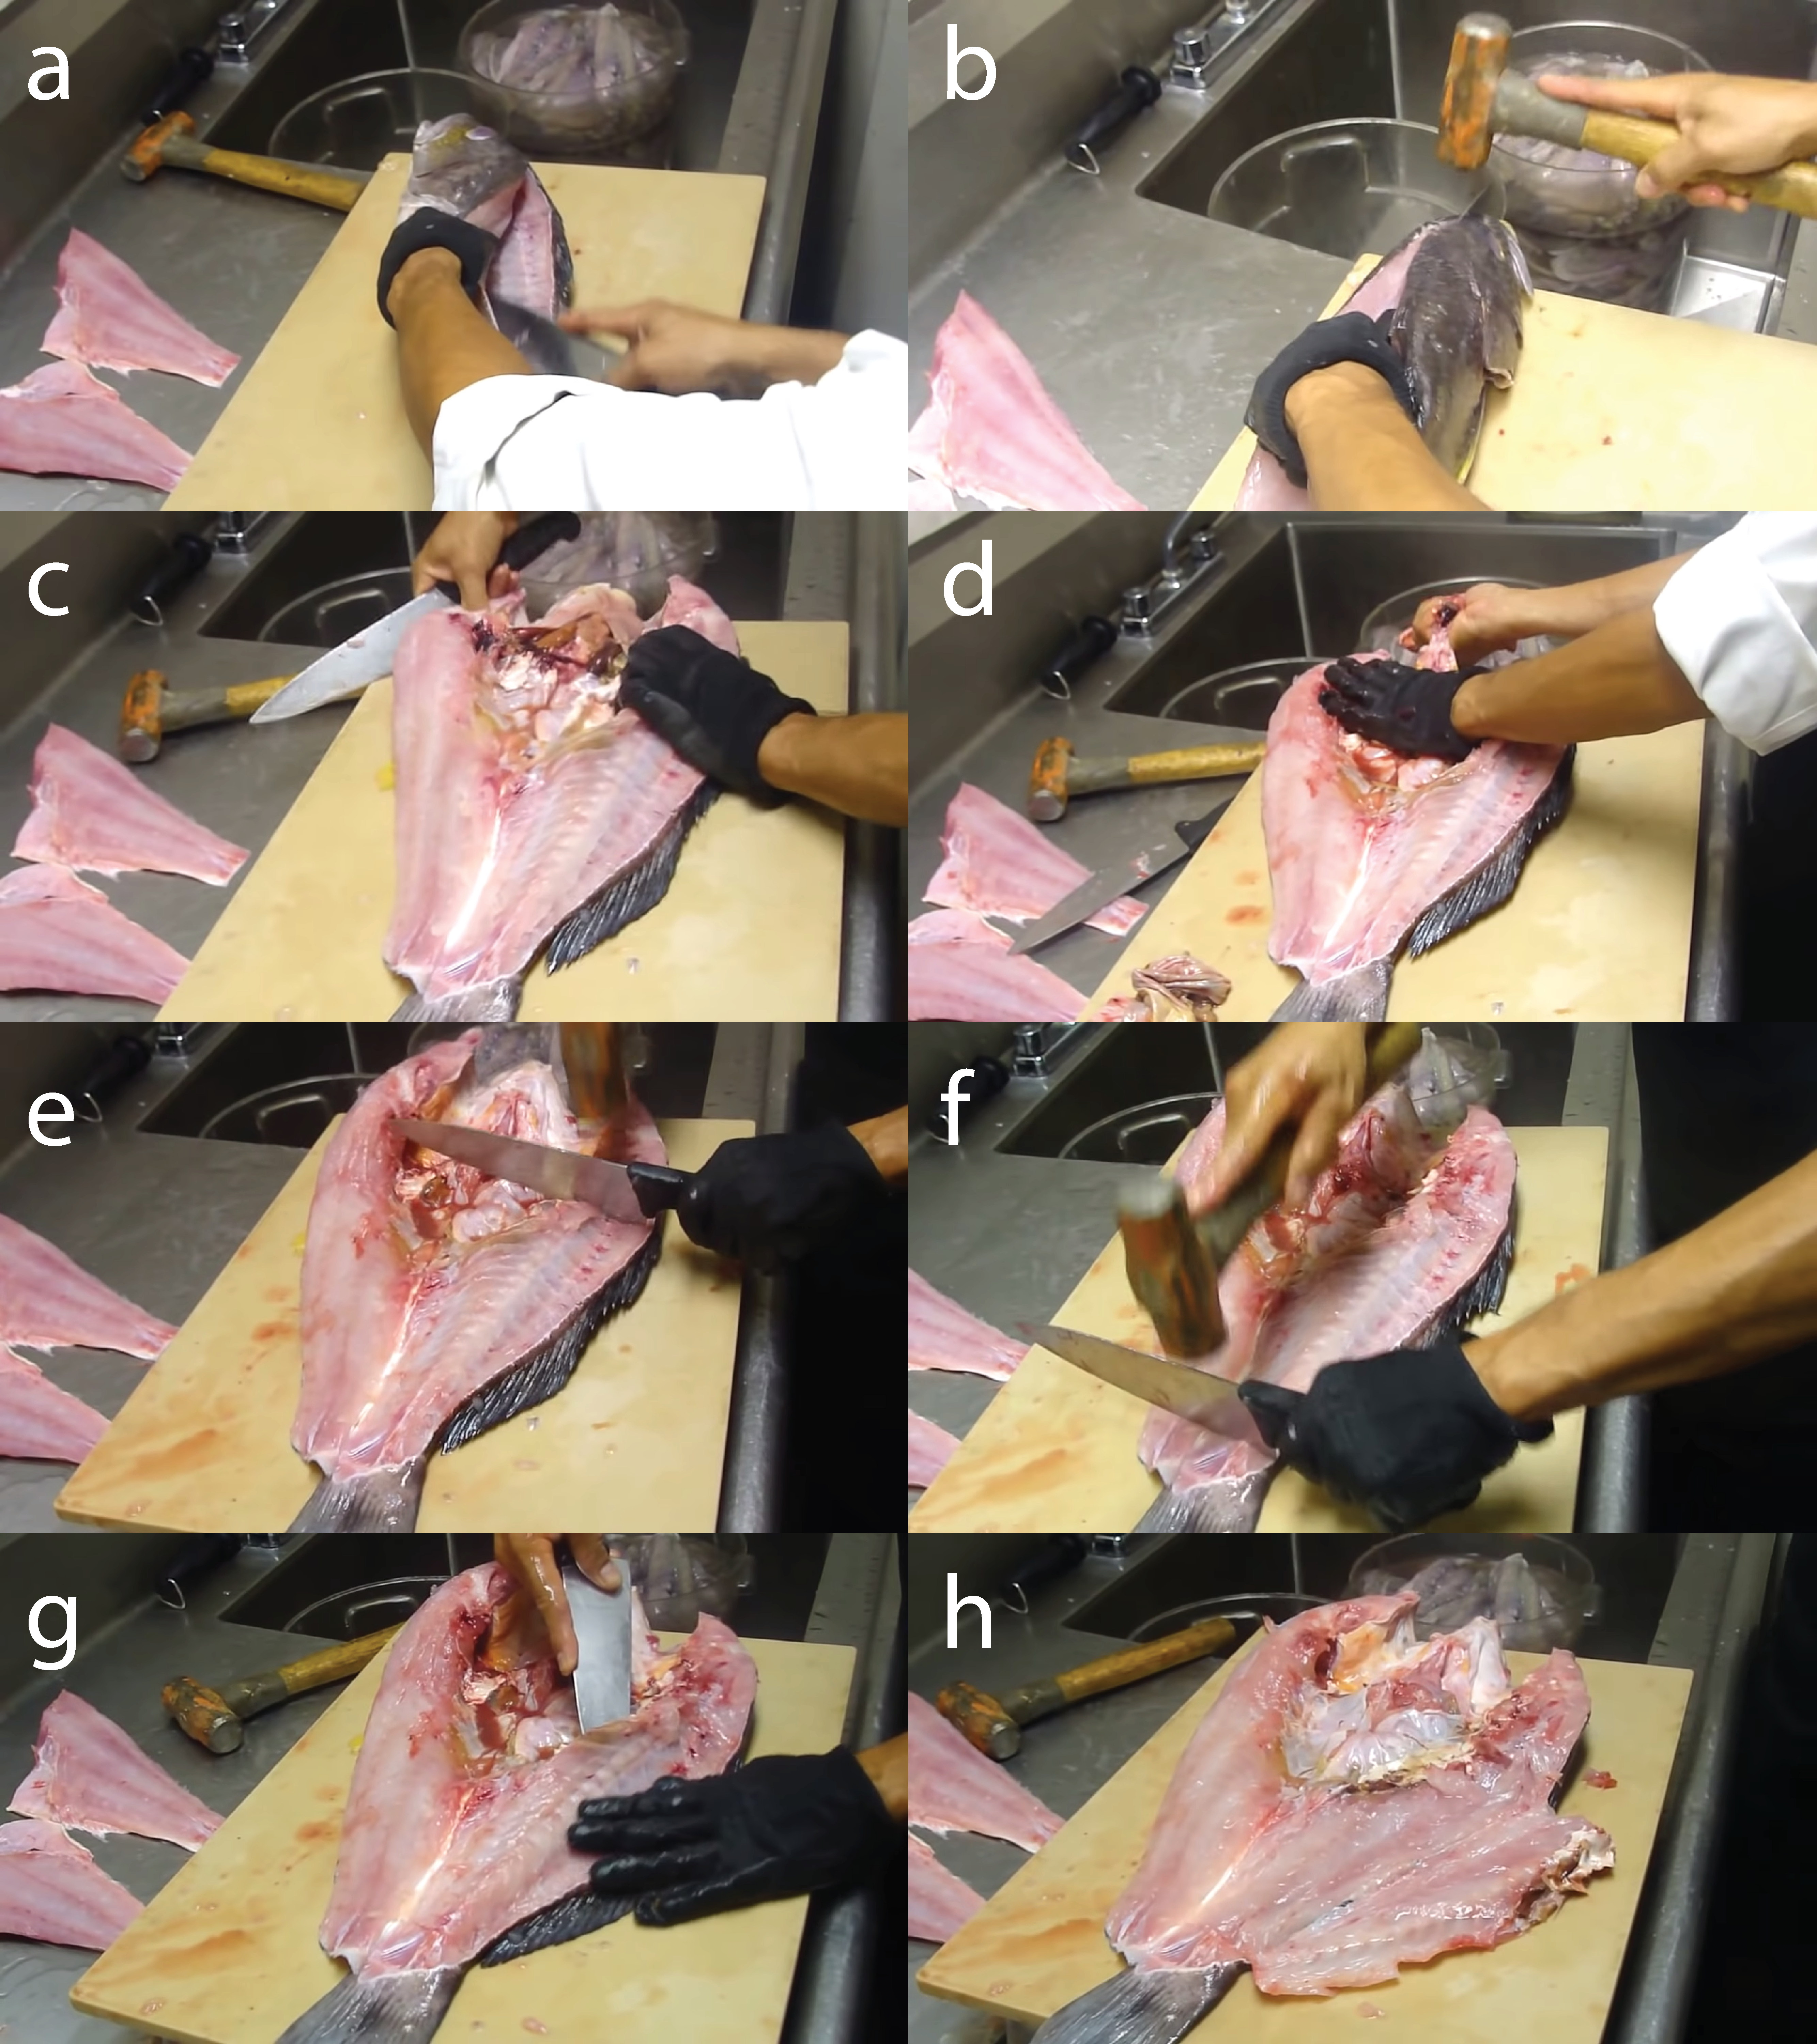
\includegraphics[width=\textwidth]{recetas/zarandeado/figuras/corte-zarandeado}
\caption{Corte de pescado para zarandear. \href{https://www.youtube.com/watch?v=_OmdFQWyWRc}{Video de Robles Ponce}}
\label{fig:corte-zarandeado}
\end{figure}